\chapter[Proposta]{Proposta}
\label{chap:Proposta}
Neste capítulo, é retomado o contexto em que o trabalho pretende contribuir, apresentando a proposta do Trabalho de Conclusão de Curso. Inicialmente na seção de \hyperref[sec:Contextualização]{Contextualização}, é 
apresentado o domínio em que o estudo está inserido. Adicionalmente, com intuito de apresentar adequadamente a aplicação, a seção \hyperref[sec:Detalhamento da Aplicacao]{Detalhamento da Aplicação} é exposta. A \hyperref[sec:Prova de Conceito]{Prova de Conceito}, 
que detalha como os testes de usabilidade serão  feitos, também é coberta no capítulo. O \hyperref[sec:Primeiro Ciclo]{Primeiro Ciclo de Teste} esclarece sobre "como"  e "o que"  foi testado, além dos resultados. Com base nos insumos obtidos no primeiro ciclo de teste, 
a seção de \hyperref[sec:Melhorias Propostas]{Melhorias Propostas} elucida sobre a incorporação das melhorias elicitadas junto ao público alvo no aplicativo em estudo, o que demandou refinamentos no protótipo de alta fidelidade, em especial no fluxo de \hyperref[sec:Onboarding]{\textit{Onboarding}}, 
e na disposição de informações em geral. O \hyperref[sec:Segundo Ciclo]{Segundo Ciclo de Teste} também é abordado, procurando mostrar os resultados obtidos com a análise da versão do aplicativo evoluída, ou seja, que teve as melhorias do primeiro ciclo incorporadas. 
Ademais, encontra-se o \hyperref[sec:Backlog]{\textit{Backlog} de Melhorias} (priorizado), no qual constam as principais funcionalidades que serão implementadas de fato no aplicativo, com base no protótipo de alta fidelidade validado em dois ciclos de teste. 
Por fim, tem-se o \hyperref[sec:Resumo Proposta]{Resumo do Capítulo}.

\section{Contextualização}
\label{sec:Contextualizacao}
O presente trabalho tem como objetivo principal investigar as melhorias na usabilidade e na experiência do usuário de um aplicativo móvel chamado Multilind, desenvolvido para o mapeamento das línguas indígenas do Brasil. 
De acordo com \citeonline{bevan1995}, usabilidade é o termo técnico usado para descrever a qualidade de uso de uma interface. Em outras palavras, refere-se à facilidade com que os usuários podem interagir e realizar 
tarefas em um sistema, aplicativo ou site. Uma interface com boa usabilidade é aquela que proporciona uma experiência fluida, intuitiva e eficiente para os usuários. Complementarmente, a experiência de usuário preocupa-se 
com as percepções e respostas do usuário antes, durante e após o uso da aplicação \cite{iso9241210}.

O Multilind foi desenvolvido em parceria com a professora Altaci Corrêa Rubim\footnote{\url{https://amazoniareal.com.br/personagem/altaci-correa-rubim/}(último acesso: Julho 2023)}, representante brasileira do Grupo de Trabalho Mundial da Década das Línguas Indígenas, 
e membros do GT do Brasil. O aplicativo foi criado durante disciplinas de Métodos de Desenvolvimento de Software e Engenharia de Produto de Software da Universidade de Brasília - Campus Gama, utilizando a licença MIT. Ele possui funcionalidades que permitem o mapeamento 
das línguas indígenas, fornecendo informações sobre cada língua, como família linguística, área de ocorrência, palavras e suas traduções.

Considerando que é uma aplicação já existente, para implementar tais melhorias, foram consideradas as heurísticas de Nielsen, que são diretrizes elaboradas para garantir que as interfaces do sistema atendam aos princípios fundamentais de usabilidade. Além disso, em um 
primeiro momento, para maior familiaridade da autora às demandas, propõe-se o uso de provas de conceitos, orientadas a ciclos de teste de usabilidade. Adiante, com o avançar do trabalho na segunda etapa do TCC, pretende-se seguir de forma mais rigorosa as etapas de 
pesquisa-ação, estabelecidas para condução da análise de resultados do trabalho com um todo. O foco das provas de conceito é o atendimento adequado das necessidades e expectativas, tanto dos usuários do aplicativo Multilind, quanto da equipe envolvida. A ideia é tratar 
demandas mais prioritárias, e não a completude das demandas. Essa decisão foi tomada considerando prazos e desenvolvimento solo da autora.

Na primeira etapa do TCC, foram desenvolvidos protótipos que permitiram a visualização e a avaliação preliminar das melhorias propostas em termos de usabilidade e experiência do usuário. Os protótipos 
foram submetidos a avaliações junto ao público alvo, permitindo, desde o começo do trabalho, ajustes e refinamentos com base no \textit{feedback} obtido. 

Uma vez cumprida com essa etapa inicial de validação dos protótipos, a segunda etapa do trabalho consistirá no desenvolvimento efetivo do aplicativo Multilind evoluído, orientando-se pelas melhorias identificadas. Com base nas lições aprendidas durante a fase de prototipação, 
funcionalidades serão implementadas, além da realização de testes mais aprofundados, a fim de garantir que a interface final do aplicativo atenda aos critérios de usabilidade e proporcione uma maior satisfação, engajamento e facilidade de uso. No intuito de conferir uma visão 
mais concreta sobre o objeto de estudo desse trabalho, segue o Detalhamento da Aplicação. Essa aplicação, na verdade, é um aplicativo e, como já revelado, chama-se Multilind.
	
\section{Detalhamento da Aplicação}
\label{sec:Detalhamento da Aplicacao}
Ressalta-se a relevância de explorar em detalhes o aplicativo Multilind, em sua versão v.1.4.0. Como a aplicação já se encontra desenvolvida, em sua primeira versão, há necessidade de conhecer e revelar sobre Arquitetura, Público-Alvo, Guia de Estilo e Funcionalidades. Esses aspectos são 
tratados na sequência. O compromisso da autora é não violar o entorno do aplicativo Multilind, sejam as expectativas dos usuários que já consomem o aplicativo, e reconhecem no mesmo funcionalidades bem ajustadas; sejam as noções técnicas, com uso de tecnologias já estabelecidas.

\subsection{Arquitetura}
\label{Arquitetura}
O projeto do aplicativo Multilind contém três repositórios principais: o respositório de \textit{Frontend}, que armazena a camada que lida com as interfaces do usuário, desenvolvido em React Native; o repositório \textit{Content Server}, que armazena os conteúdos do sistema 
utilizando PostgreSQL, e o repositório \textit{Files Server}, responsável por armazenar e administrar os arquivos de mídia do aplicativo. Os diagramas de  pacotes, correspondentes a cada repositório, podem ser conferidos nas Figuras \ref{fig08}, \ref{fig09} e \ref{fig10}.

\begin{figure}[h!]
	\centering
	\caption{Diagrama de Pacotes \textit{Content Server}}
	\resizebox{0.8\textwidth}{!}{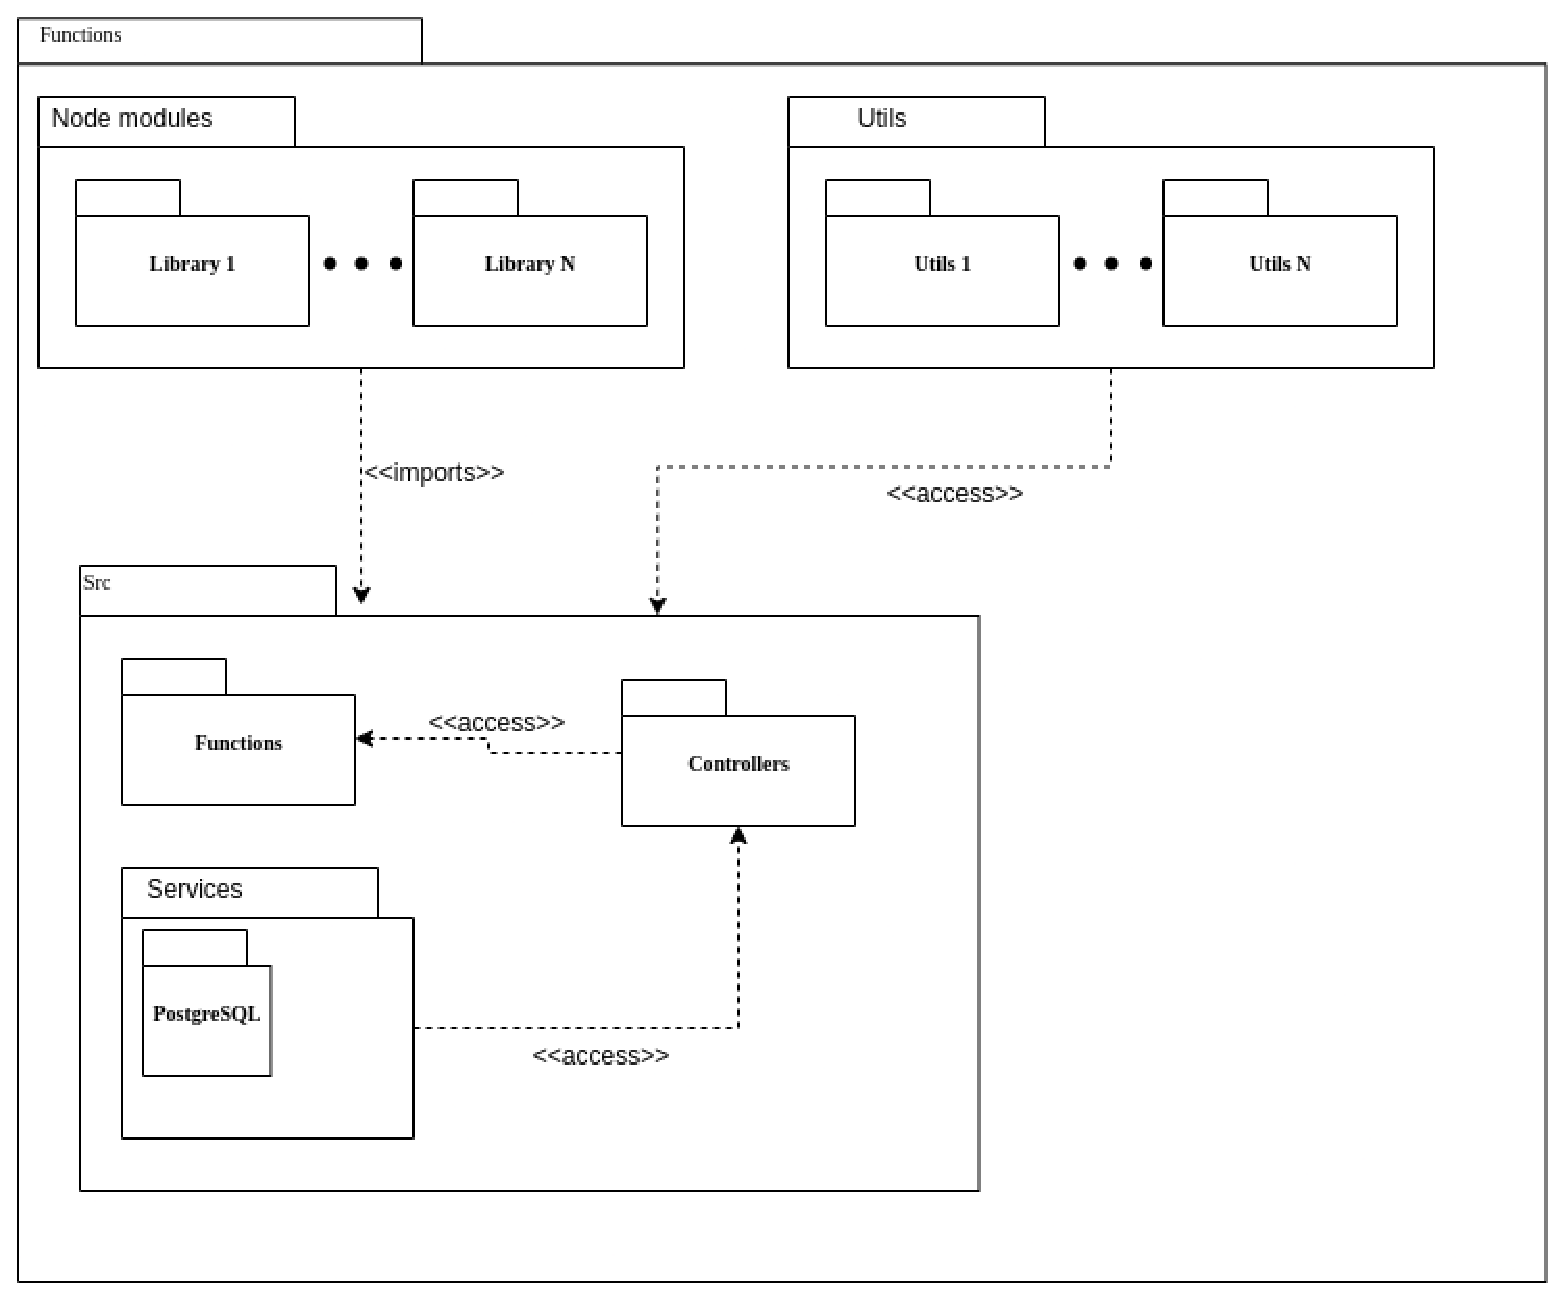
\includegraphics{figuras/content.eps}}
	\begin{tablenotes}[flushleft]
		\centering
		\item \textit{Fonte:} Multilind.
	\end{tablenotes}
	\label{fig08}
\end{figure}
\begin{figure}[h!]
	\centering
	\caption{Diagrama de Pacotes \textit{Frontend}}
	\resizebox{0.6\textwidth}{!}{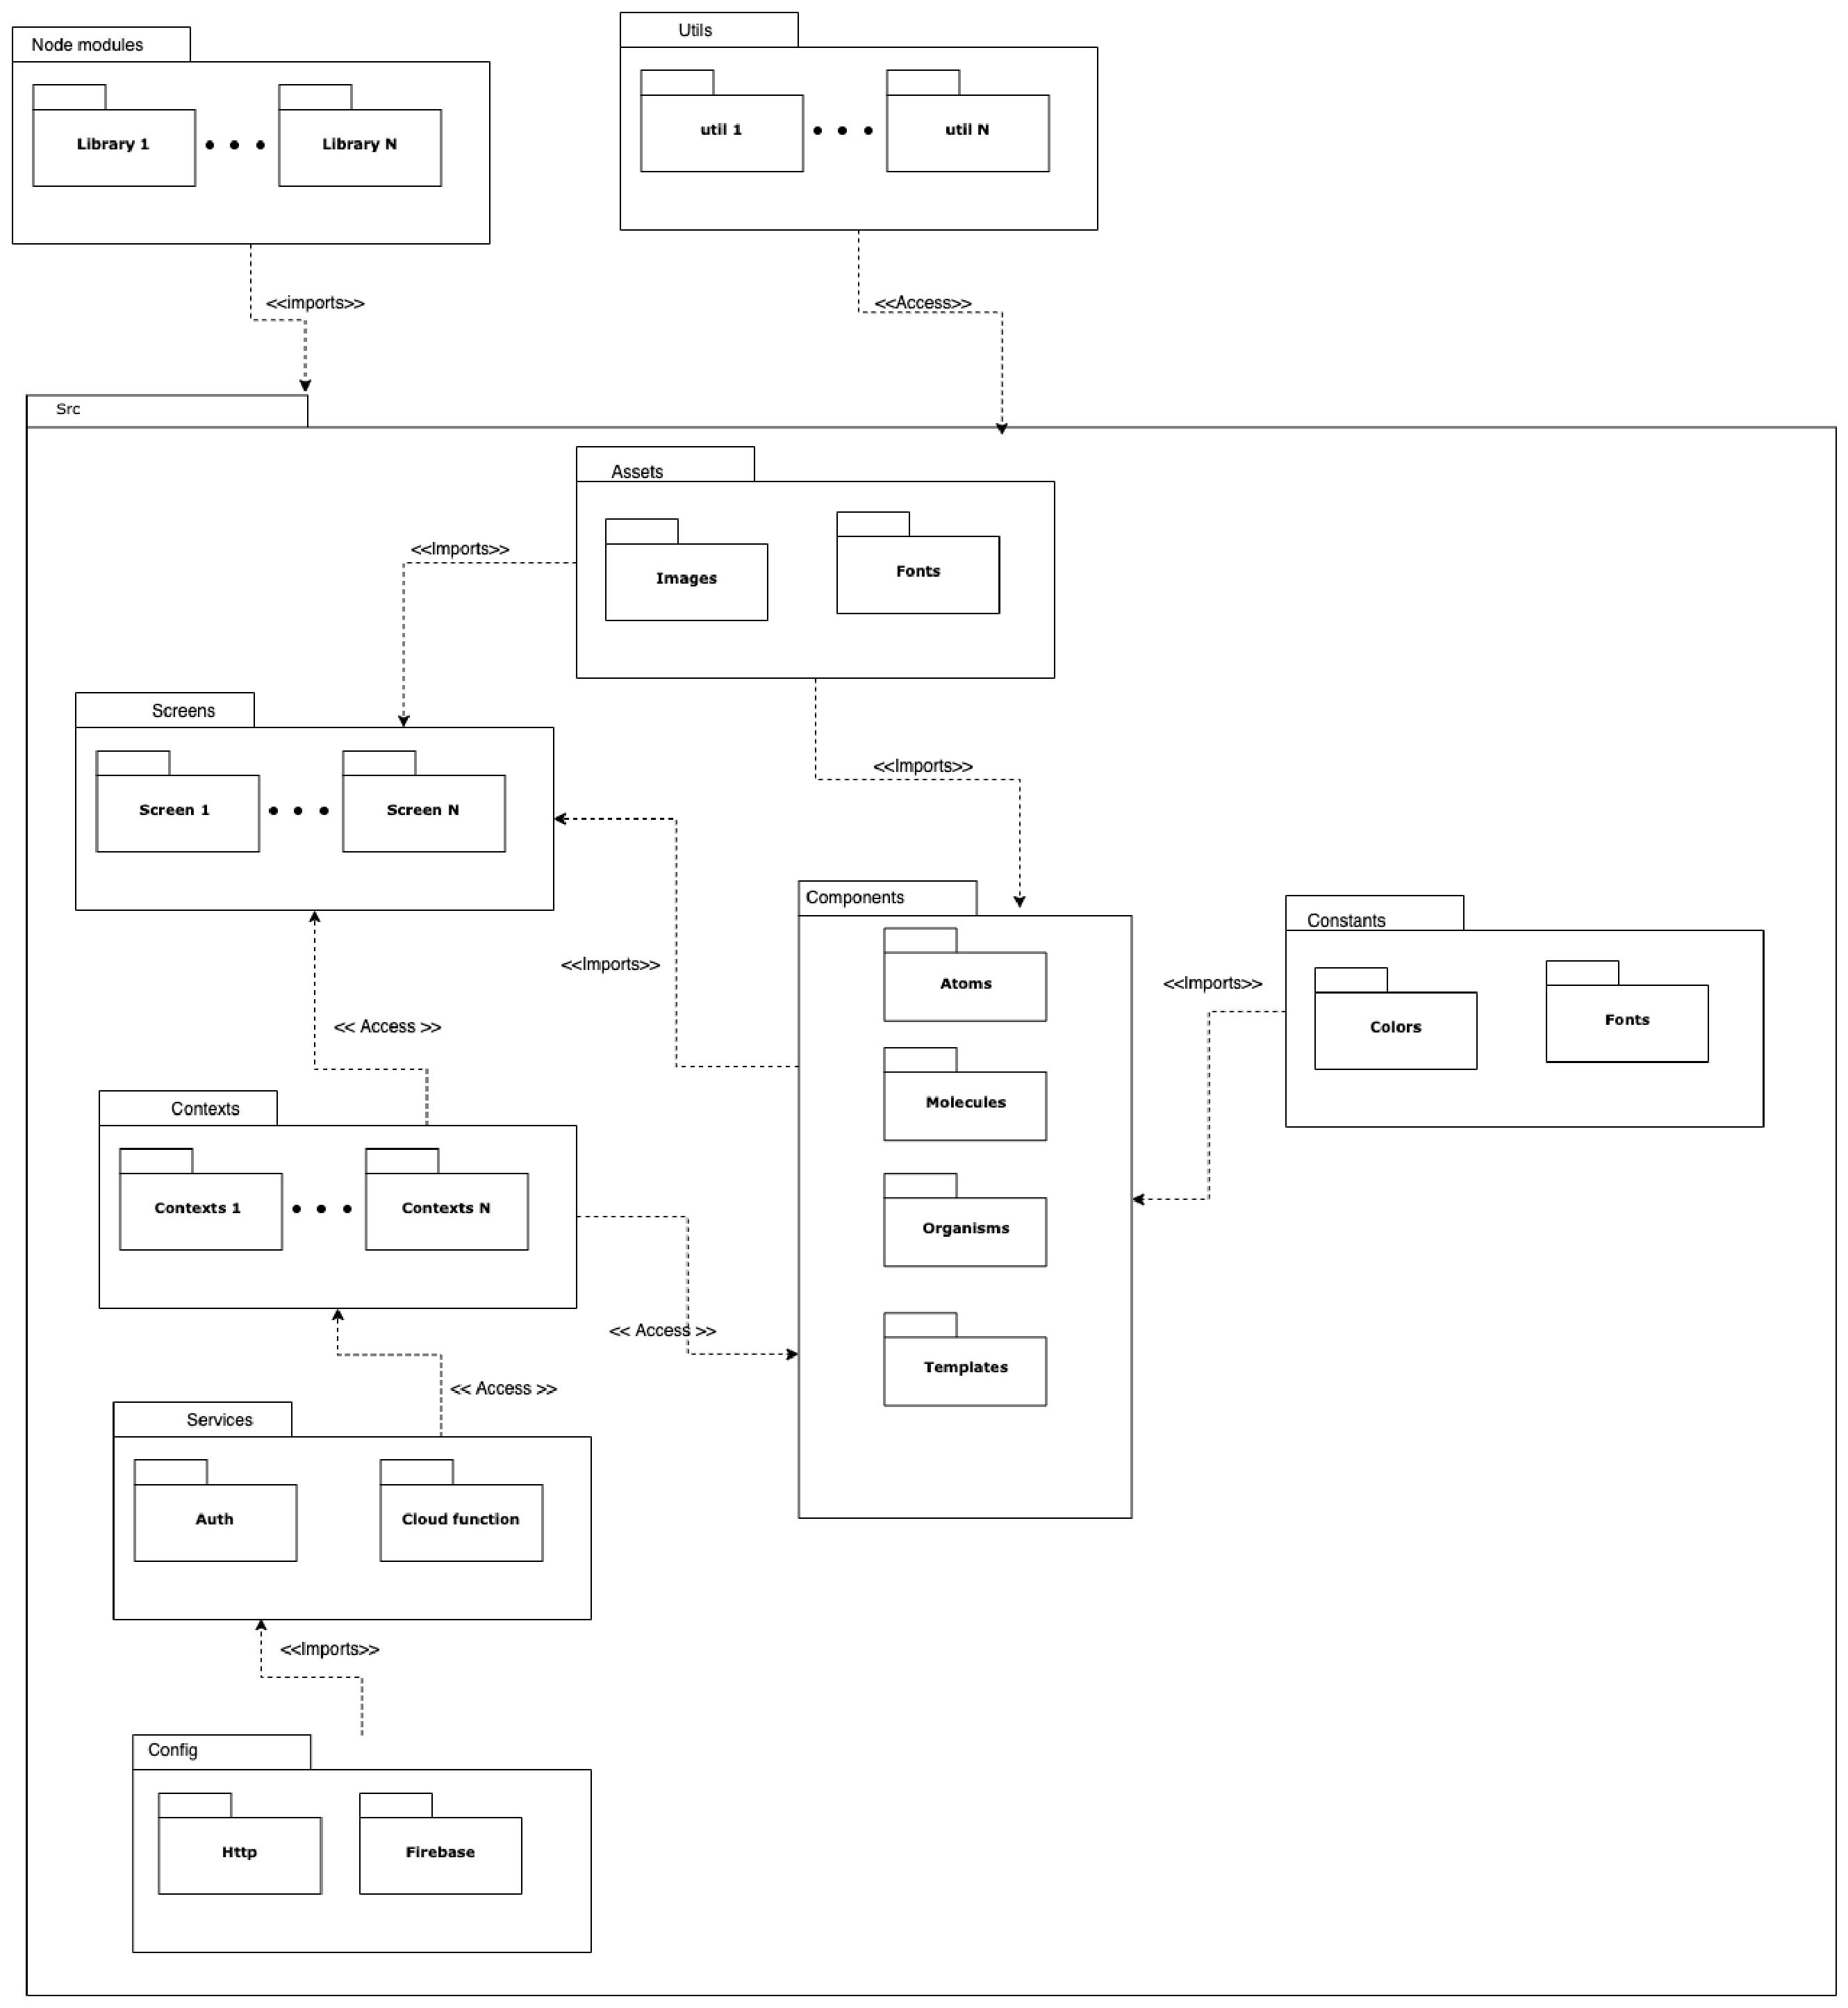
\includegraphics{figuras/frontend.eps}}
	\begin{tablenotes}[flushleft]
		\centering
		\item \textit{Fonte:} Multilind.
	\end{tablenotes}
	\label{fig09}
\end{figure}

\begin{figure}[h!]
	\centering
	\caption{Diagrama de Pacotes \textit{Files Server}}
	\resizebox{0.5\textwidth}{!}{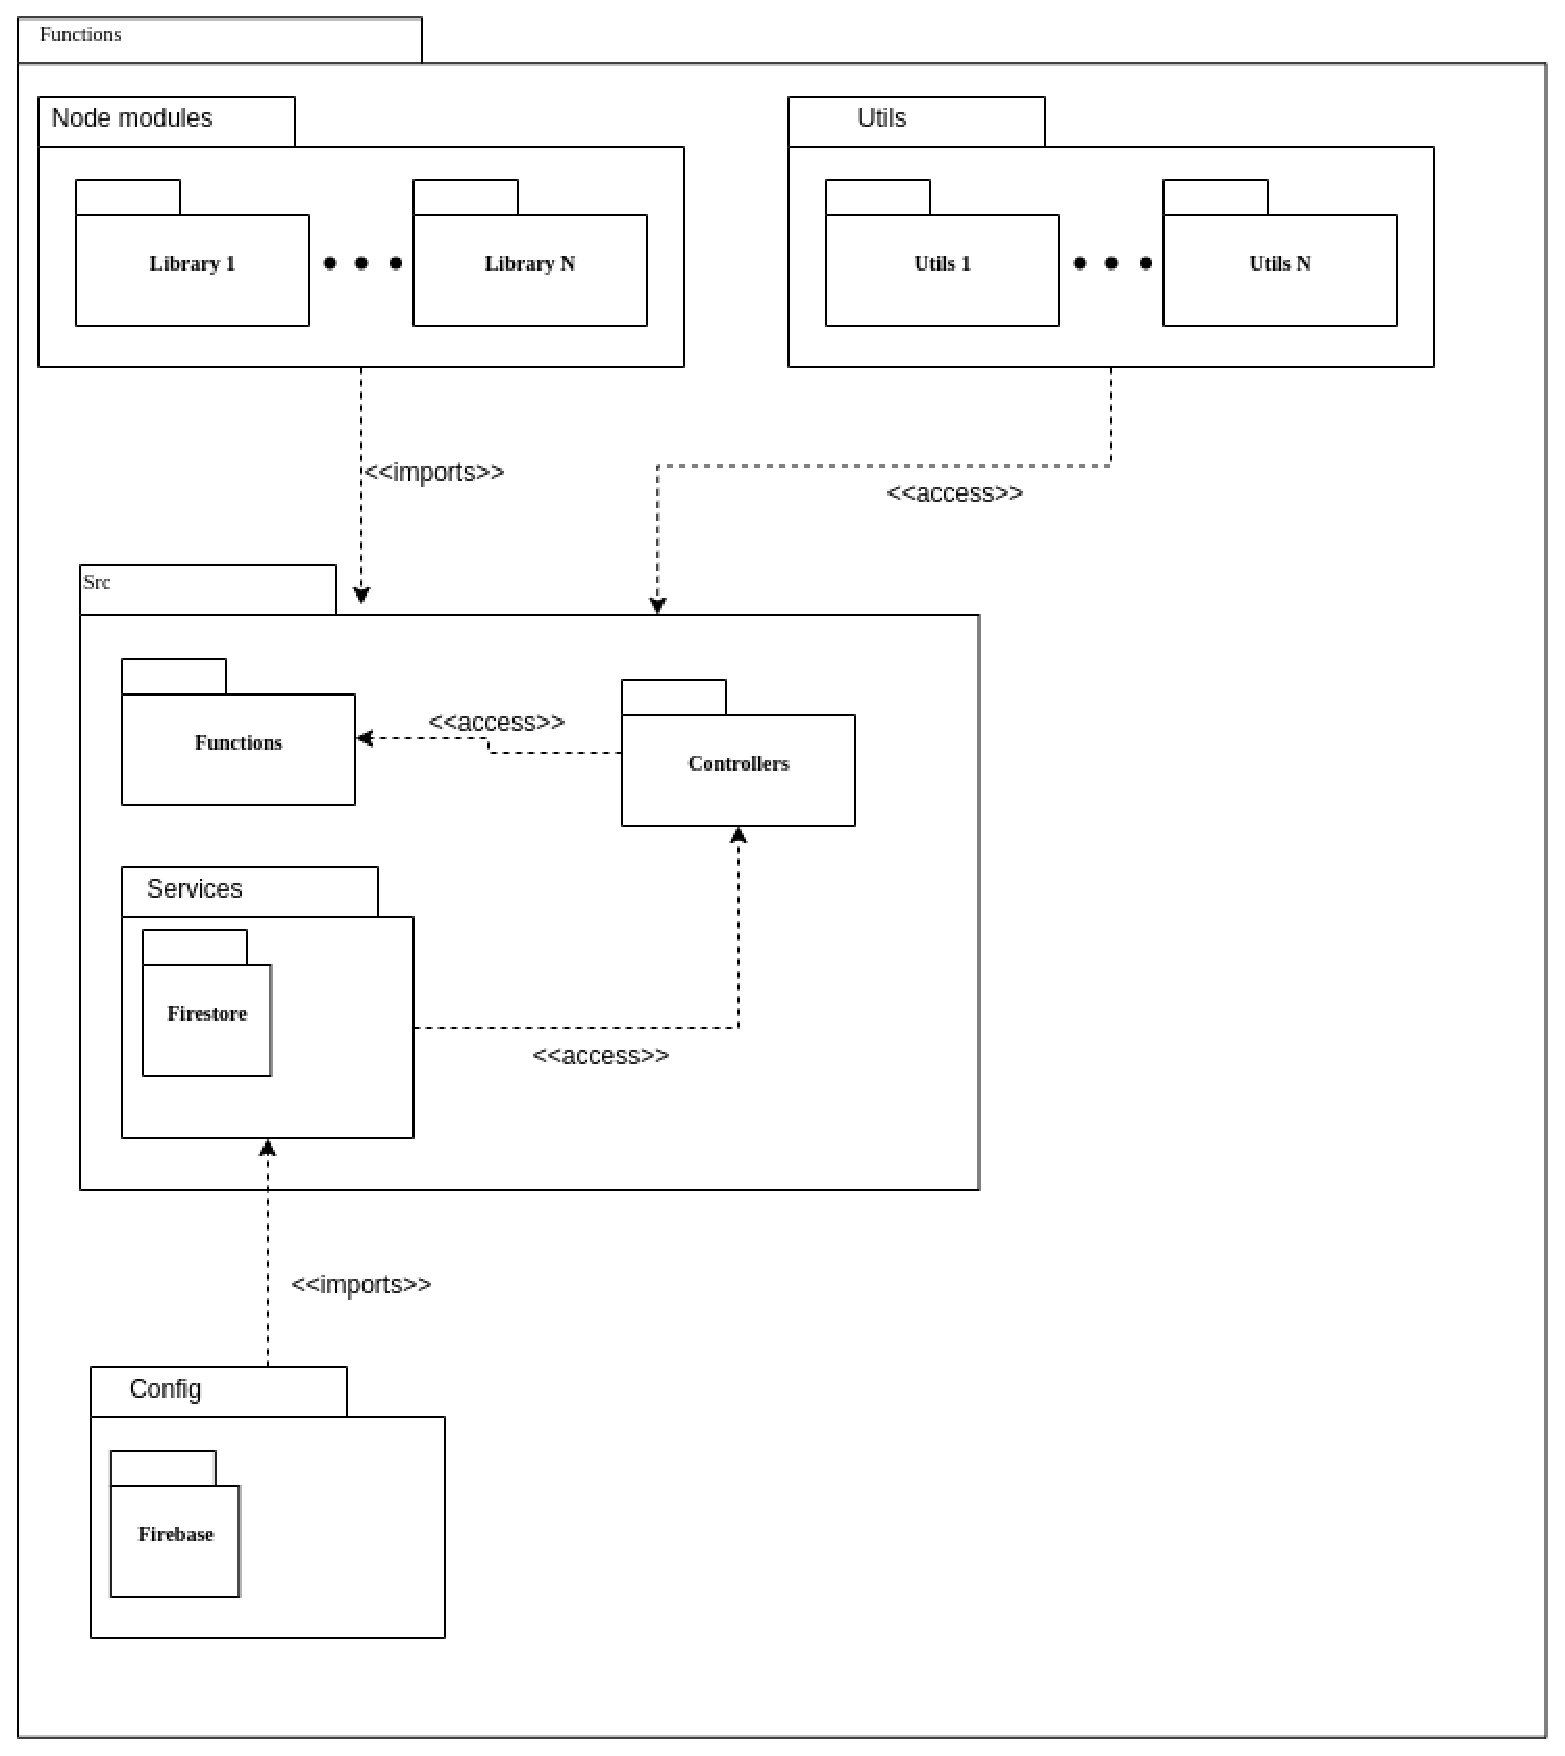
\includegraphics{figuras/assets.eps}}
	\begin{tablenotes}[flushleft]
		\centering
		\item \textit{Fonte:} Multilind.
	\end{tablenotes}
	\label{fig10}
\end{figure}

\subsection{Público-Alvo}
\label{Publico-Alvo}
A Lean Inception, criada por \citeonline{lean}, foi utilizada como forma de alinhar os desenvolvedores e \textit{stakeholders} em relação ao aplicativo, antes de sua execução, e confirmar sua viabilidade e sua necessidade. O processo aborda a visão do produto; a compreensão de personas; suas jornadas de usuário, e 
o desenvolvimento de funcionalidades de alto nível \cite{lean}. No estágio de definição da visão do produto, a equipe e os \textit{stakeholders} do projeto responderam questões relativas ao público alvo da aplicação; o objetivo, e as principais características, como pode ser visto nas 
Figuras \ref{fig11} e \ref{fig12}. Ambas as imagens são autoexplicativas. Entretanto, é pertinente mencionar, com base na Figura \ref{fig11}, sobre o foco do produto em povos indígenas e todos que possuem interesse sobre linguas indígenas; bem como em aspectos qualitativos, tais como: praticidade, acessibilidade, atualidade 
e disponibilidade. Na Figura \ref{fig12}, estrutura-se a definição do produto considerando: "É", com destaque em é interativo, prático, mobile, gratuíto, dentre outros; "NÃO É", mencionando que não é jogo, rede social, chat, site, blog ou fórum, tampouco complexo; "FAZ", com menção a fazer mapeamento de línguas, 
pesquisa por palavras, dentre outros; "NÃO FAZ", destancando que não faz restrição ao acesso à informação, nem expõe dados pessoais, dentre outros.

\begin{figure}[h!]
	\centering
	\caption{Visão de Produto}
	\resizebox{0.85\textwidth}{!}{\includegraphics{figuras/visao_produto.eps}}
	\begin{tablenotes}[flushleft]
		\centering
		\item \textit{Fonte:} Multilind.
	\end{tablenotes}
	\label{fig11}
\end{figure}

\begin{figure}[h!]
	\centering
	\caption{Definição do Produto}
	\resizebox{1\textwidth}{!}{\includegraphics{figuras/produto_e_nao_e.eps}}
	\begin{tablenotes}[flushleft]
		\centering
		\item \textit{Fonte:} Multilind.
	\end{tablenotes}
	\label{fig12}
\end{figure}

Como definidas no Capítulo de \hyperref[chap:Referencial]{Referencial Teórico}, as personas são representações detalhadas de perfis semifictícios, sendo desenvolvidas para ajudar a equipe na melhor compreensão sobre os usuários, bem 
como sobre suas necessidades e expectativas. 

Ainda durante a Lean Inception, na fase de descrição de personas, foram criadas três personas que representam diferentes tipos de usuários do aplicativo. Essas personas foram essenciais para realizar as jornadas das personas, e levantar as 
funcionalidades necessárias para atender às necessidades e expectativas dos envolvidos. As Figuras \ref{fig13}, \ref{fig14} e \ref{fig15} mostram os três principais perfis levantados.

\begin{figure}[h!]
	\centering
	\caption{Persona 1}
	\begin{adjustbox}{center}
		\includegraphics[width=1.1\textwidth]{figuras/persona1.eps}
	\end{adjustbox}
	\begin{tablenotes}[flushleft]
		\centering
		\item \textit{Fonte:} Autora.
	\end{tablenotes}
	\label{fig13}
\end{figure}

\begin{figure}[h!]
	\centering
	\caption{Persona 2}
	\begin{adjustbox}{center}
		\includegraphics[width=1.1\textwidth]{figuras/persona2.eps}
	\end{adjustbox}
	\begin{tablenotes}[flushleft]
		\centering
		\item \textit{Fonte:} Autora.
	\end{tablenotes}
	\label{fig14}
\end{figure}

\begin{figure}[h!]
	\centering
	\caption{Persona 3}
	\begin{adjustbox}{center}
		\includegraphics[width=1.5\textwidth]{figuras/persona3.eps}
	\end{adjustbox}
	\begin{tablenotes}[flushleft]
		\centering
		\item \textit{Fonte:} Autora.
	\end{tablenotes}
	\label{fig15}
\end{figure}

\subsection{Guia de Estilo}
\label{Guia de Estilo}
O guia de estilo do produto foi desenvolvido a partir da criação de um Manual de Identidade Visual\footnote{Manual de Identidade Visual Multilind, 2021. Disponível
em: \url{https://fga-eps-mds.github.io/2021.1-Multilind-Docs/img/manualIdentidade/Manual_Id.pdf} (último acesso: Julho 2023)}. Esse manual definiu os elementos fundamentais da marca, incluindo cores, tipografia, aplicação da marca, símbolo e conceitos base.

O símbolo do Multilind é representado pelo beija-flor, que simboliza a pajé e a espiritualidade da língua. As principais cores presentes na logomarca são representadas pelos hexadecimais "\#04B47F" e "\#338BAE".

Além disso, outras cores foram selecionadas como base para o desenvolvimento do \textit{design} de interface da aplicação, que podem ser vistas nas Figuras \ref{fig16} e \ref{fig17}.

\begin{figure}[h!]
	\centering
	\caption{Paleta de Cores - Verde}
	\resizebox{1\textwidth}{!}{\includegraphics{figuras/cor1.eps}}
	\begin{tablenotes}[flushleft]
		\centering
		\item \textit{Fonte:} Autora.
	\end{tablenotes}
	\label{fig16}
\end{figure}

\begin{figure}[h!]
	\centering
	\caption{Paleta de Cores - Azul}
	\resizebox{1\textwidth}{!}{\includegraphics{figuras/cor2.eps}}
	\begin{tablenotes}[flushleft]
		\centering
		\item \textit{Fonte:} Autora.
	\end{tablenotes}
	\label{fig17}
\end{figure}

\subsection{Funcionalidades}
\label{Funcionalidades}
A versão 1.4.0 da aplicação possui diversas funcionalidades voltadas para o mapeamento e a divulgação das línguas indígenas brasileiras. Entre essas funcionalidades, destaca-se o mapeamento das línguas, que permite aos usuários 
explorar através do mapa e descobrir informações sobre línguas indígenas brasileiras. Isso inclui detalhes sobre o tronco e a família linguística à qual a língua pertence, seu dicionário e imagens relativas à lista de palavras.

Além disso, a aplicação também oferece recursos de tradução para o português indígena e o português formal. Os usuários podem fazer buscas por palavras e visualizar informações como significado e imagens relativas. Um levantamento 
mais pleno sobre essas funcionalidades pode ser obtido consultando o repositório do aplicativo Multilind. Nesse repositório, a equipe procurou destacar sobre os principais propósitos do aplicativo. \footnote{Repositório Multilind, 2023. Disponível
em: \url{https://fga-eps-mds.github.io/2021.1-Multilind-Docs/} (último acesso: Julho 2023)}

\begin{figure}[h!]
	\centering
	\caption{Telas da Aplicação - Mapa e Palavra Específica}
	\resizebox{1\textwidth}{!}{\includegraphics{figuras/app1.eps}}
	\begin{tablenotes}[flushleft]
		\centering
		\item \textit{Fonte:} Autora.
	\end{tablenotes}
	\label{fig18}
\end{figure}

\begin{figure}[h!]
	\centering
	\caption{Telas da Aplicação - Línguas e Dicionário}
	\resizebox{1\textwidth}{!}{\includegraphics{figuras/app2.eps}}
	\begin{tablenotes}[flushleft]
		\centering
		\item \textit{Fonte:} Autora.
	\end{tablenotes}
	\label{fig19}
\end{figure}


\section{Prova de Conceito}
\label{sec:Prova de Conceito}
Com o objetivo de avaliar o aplicativo Multilind em relação a usabilidade e experiência de usuário, provas de conceito foram 
realizadas para avaliar tanto a última versão do aplicativo (v1.4.0), quanto a versão com melhorias propostas, com cinco usuários diferentes.

A escolha de cinco usuários é uma abordagem amplamente adotada, \citeonline{usabilitytest} argumenta que realizar testes com cinco usuários é suficiente para identificar a maioria dos problemas de 
usabilidade. Ele baseia essa conclusão em estudos empíricos e observações, sugerindo que a descoberta de problemas de usabilidade tende a estagnar após o quinto participante, com poucos benefícios 
adicionais sendo obtidos com participantes adicionais.

O primeiro ciclo de testes foi realizado com objetivo de coletar métricas e informações de usabilidade e experiência do usuário. Já o segundo ciclo de testes visa validar as melhorias propostas e 
avaliar seus resultados. Todos os testadores participaram voluntariamente, de acordo com os termos estabelecidos no Termo de Consentimento, que foi adaptado do 
modelo da Universidade de Araraquara (Universidade de Araraquara, 2023), disponível no Apêndice B para consulta.
 
\section{Primeiro Ciclo de Testes}
\label{sec:Primeiro Ciclo}
O primeiro ciclo de testes de usabilidade foi realizado com cinco testadores, que fazem parte do público alvo da aplicação. Foi realizado um teste abrangendo as sete funcionalidades 
principais do aplicativo, com o objetivo de identificar seus aspectos-chave. Durante o teste, os usuários forneceram \textit{feedback} instantâneo sobre sua percepção de cada funcionalidade testada. 

Além disso, como uma ferramenta de teste de usabilidade, o Maze foi utilizado para avaliar a navegação e a facilidade de uso do aplicativo. Os testadores foram solicitados a realizar  
tarefas no protótipo\footnote{Protótipo Versão 1.4.0. Disponível em: \url{https://shorturl.at/DGHKU}(último acesso: Julho 2023)} 
e o tempo necessário para concluir o percurso foi registrado. Essa abordagem permitiu identificar eventuais dificuldades de navegação e fornecer informações para aprimorar a usabilidade do aplicativo. Após a conclusão dos 
testes, foi aplicado um questionário baseado no Formulário de \textit{Attrakdiff} para avaliar a experiência do usuário no aplicativo Multilind.

\begin{description}
    \item As funcionalidades testadas foram:
	\begin{itemize}
		\item F01 - Visualizar línguas através do mapa
		\item F02 - Ver detalhes de uma língua ao clicar em um ponto no mapa
		\item F03 - Visualizar línguas por ordem alfabética
		\item F04 - Visualizar línguas por família linguística
		\item F05 - Ver dicionário de palavras de uma língua específica
		\item F06 - Ver tradução de uma palavra para o português formal
		\item F07 - Visualizar imagens relativas as palavras de uma língua
	\end{itemize}
\end{description}

\subsubsection{Resultado do Primeiro Ciclo de Testes}
\label{sec:Resultado do Primeiro Ciclo de Testes}
Após finalizar o primeiro ciclo de testes, utilizando a versão mais recente da aplicação, alguns \textit{feedbacks} foram realizados pelos testadores, que incluem:

\begin{itemize}
	\item Falta de orientação no primeiro uso: foi observado pelos testadores uma falta de instruções claras e orientações sobre como navegar e utilizar as funcionalidades no primeiro acesso ao aplicativo.
	\item Maior clareza na opção de visualizar línguas por família linguística: alguns testadores relataram dificuldades em localizar a opção para visualizar as línguas agrupadas por família linguística.
	\item Ausência de cores: usuários relataram sentir que a aplicação carecia de uma paleta de cores mais vibrantes para torná-la visivelmente atraente.
	\item Carência de informações a respeito de contribuição: houve interesse manifestado por alguns testadores em contribuir com a base de dados do aplicativo, porém, sentiram falta de informações a respeito 
	de como contribuir no aplicativo.
\end{itemize}

A Tabela \ref{tab06} apresenta o tempo gasto por cada testador durante o teste de usabilidade separado por funcionalidade.

\begin{table}[h!]
	\centering
	\caption{Tempo gasto por testador - Primeiro ciclo de testes}
	\label{tab06}
	\begin{tabular}{l|l|l|l|l|l}
	\hline
	Fucionalidade & Testador 1 & Testador 2 & Testador 3 & Testador 4 & Testador 5 \\ 	\hline
	F01                   & 25.7s     & 109.3s     & 3.36s      & 232s       & 6.4s      \\
	F02                   & 21.2s        & 18.9s      & 6.45s      & 181.7s    & 17.2s     \\
	F03                   & 26.1s        & 25.7s      & 26.5s      & 36.9s     & 23.6s     \\
	F04                   & 69.6s        & 309.3s     & 283.2s     & 136.2s     & 193.9s     \\
	F05                   & 32.1s      & 31.4s      & 21.7s     & 72.6s     & 16.4s     \\
	F06                   & 30.7s     & 8.4s      & 24s     & 45.7s     & 75.5s     \\
	F07                   & 43.2s     & 23.8s      & 43.5s     & 181.2s    & 35s      \\ 	\hline
	\end{tabular}
	\begin{tablenotes}[flushleft]
		\centering
		\item \textit{Fonte:} Maze. Disponível em: \url{https://app.maze.co/report/Multilind/3nsxpiljsgn073/intro}.
	  \end{tablenotes}
\end{table}


A tabela presente no Google Sheets apresenta as avaliações obtidas por meio do formulário \textit{Attrakdiff} aplicado aos testadores do aplicativo. Além disso, as Figuras \ref{fig21} e \ref{fig22} ilustram a média de respostas geral e a média 
de respostas separadas pelas quatro dimensões principais, respectivamente.

\begin{figure}[h!]
	\centering
	\caption{Média Geral \textit{Attrakdiff} - Primeiro Ciclo de Testes}
	\resizebox{0.8\textwidth}{!}{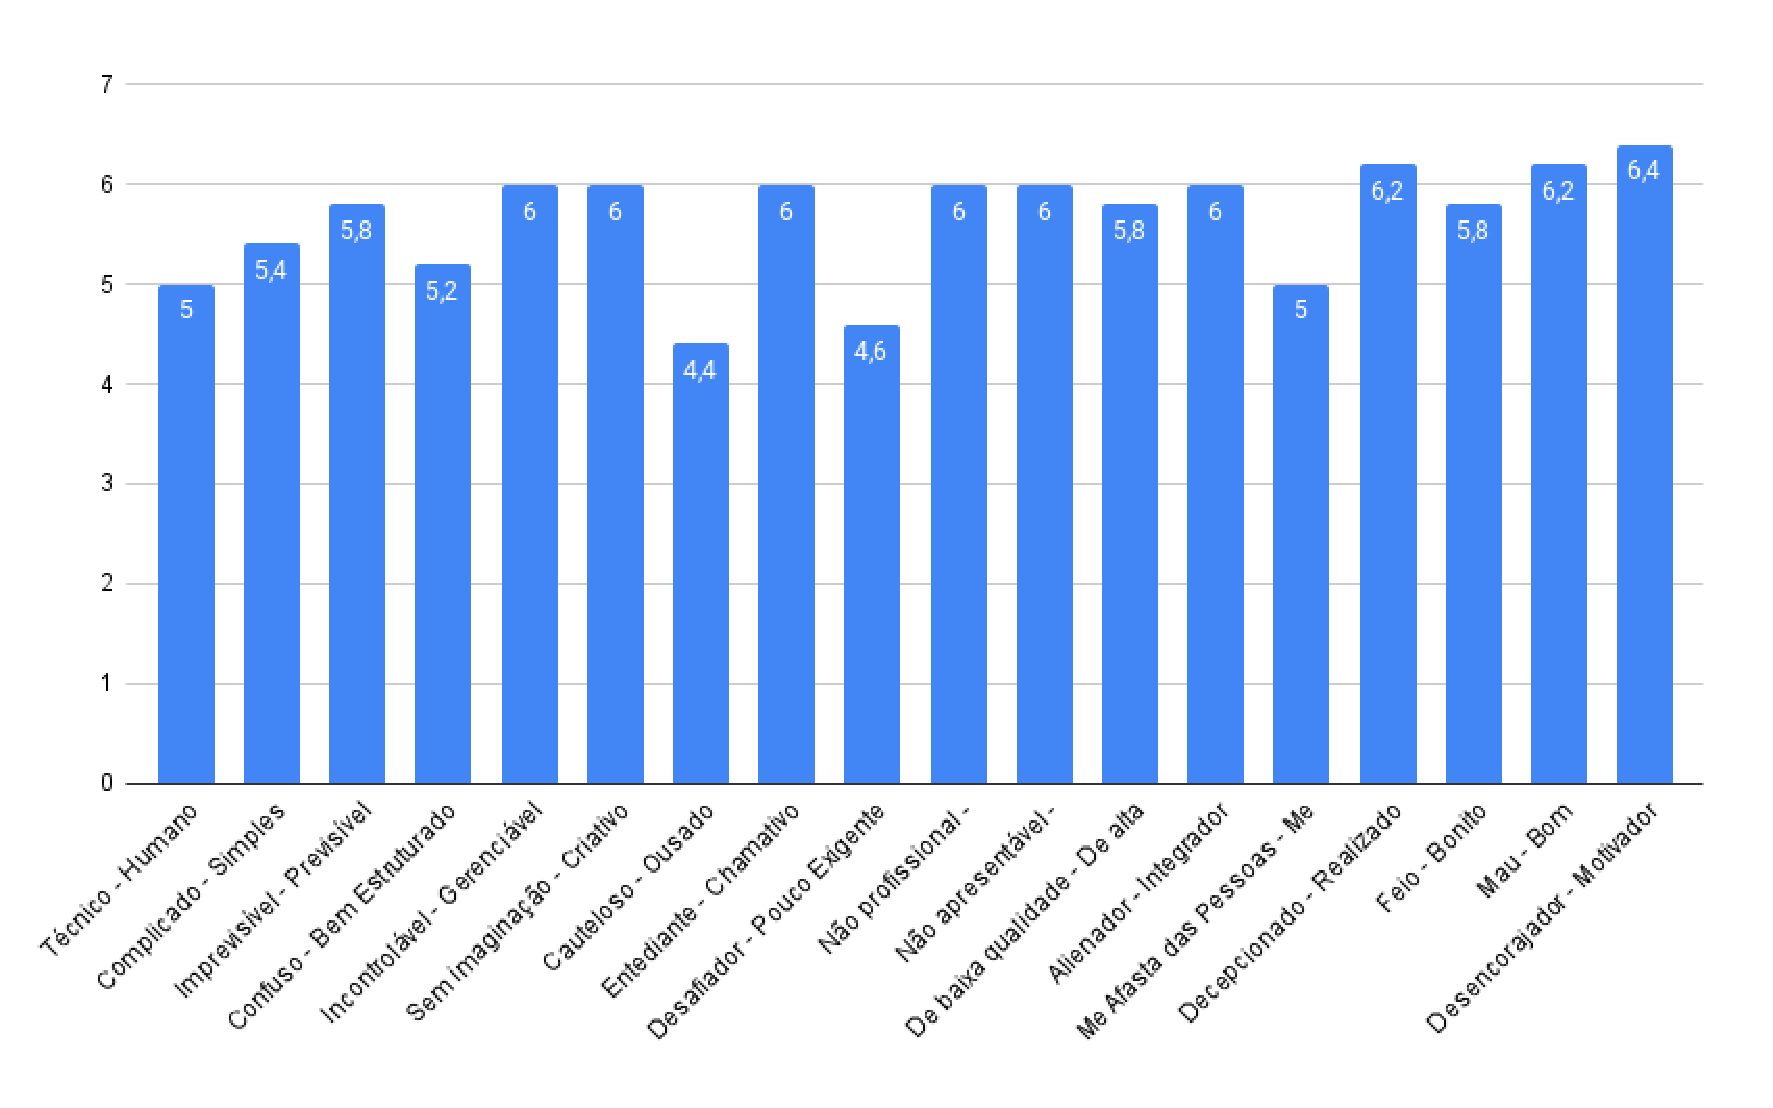
\includegraphics{figuras/media-geral.eps}}
	\begin{tablenotes}[flushleft]
		\centering
		\item \textit{Fonte:} Autora.
	\end{tablenotes}
	\label{fig20}
\end{figure}

\begin{figure}[h!]
	\centering
	\caption{Média \textit{Attrakdiff} por dimensões - Primeiro Ciclo de Testes}
	\resizebox{0.8\textwidth}{!}{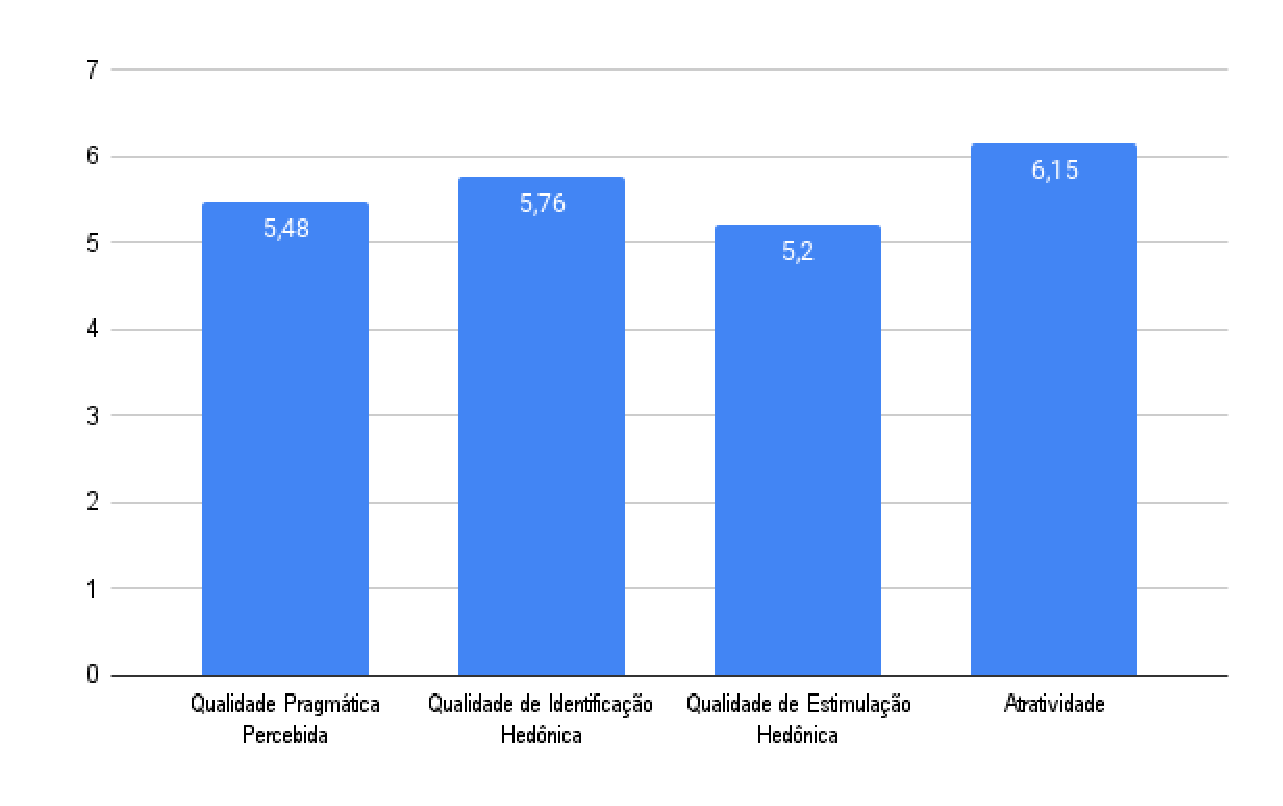
\includegraphics{figuras/media-separada.eps}}
	\begin{tablenotes}[flushleft]
		\centering
		\item \textit{Fonte:} Autora.
	\end{tablenotes}
	\label{fig21}
\end{figure}

\section{Melhorias Propostas}
\label{sec:Melhorias Propostas}
Ao buscar realizar melhorias na aplicação e reconhecendo a importância de envolver usuários reais nas tomadas de decisões, testes de usabilidade foram feitos e \textit{feedbacks} coletados, 
o que orientou o processo de melhoria de usabilidade e experiência de usuário. Bem como a aplicação das heurísticas de Nielsen que resultaram no prótotipo com melhorias\footnote{Protótipo 
com melhorias. Disponível em: \url{https://shorturl.at/ryEOR}(último acesso: Julho 2023)} que serão apresentadas nesta seção.

\subsection{\textit{Onboarding}}
\label{sec:Onboarding}
De acordo com \citeonline{cooper2007}, o objetivo do \textit{design} depende do contexto - quem são os usuários, o que estão fazendo e seus objetivos. E que não é possível criar um bom design 
seguindo regras desconectadas dos objetivos e necessidades dos usuários do seu produto. 

Com base nisso, e baseado na falta de introdução de contexto, apontada por alguns usuários como ponto de 
melhoria, foi introduzido um processo de familiarização. Tal processo, conhecido como \textit{onboarding}, pode ser entendido como a combinação de métodos e elementos que auxiliam um novo usuário 
a se familiarizar com um produto digital, seja ele um baseado na web ou aplicativo móvel. Pode incluir tutoriais interativos, orientações passo a passo, dicas contextuais e outras abordagens que 
visam orientar os usuários durante a primeira interação com o produto. Seu objetivo é permitir que os usuários compreendam como utilizar as funcionalidades do produto e alcancem seus 
objetivos de forma eficaz, reduzindo a curva de aprendizado \cite{renz2014}.

\begin{figure}[h!]
	\centering
	\caption{\textit{Onboarding}}
	\resizebox{1\textwidth}{!}{\includegraphics{figuras/onboarding.eps}}
	\begin{tablenotes}[flushleft]
		\centering
		\item \textit{Fonte:} Autora.
	\end{tablenotes}
	\label{fig22}
\end{figure}

A implementação de \textit{onboarding} colabora com algumas heurísticas, como "Visibilidade do status do sistema", pois em cada passo apresentado é possível visualizar indicador de progresso, ou seja, 
o usuário possui clareza de onde está e quantos passos restantes possui. É possível destacar, ainda, a "Correspondência entre o sistema e o mundo real", utilizando termos e elementos que os usuáŕios 
possuem familiaridade, facilitando o processo de integração. Em relação ao "Controle e liberdade do usuário", opções para avançar, voltar e pular o processo são fornecidas. Além disso, "Consistência e 
padrões" foram seguidos, utilizando componentes reutilizáveis e garantindo a consistência. E por fim, a "Prevenção de erros", por incluir dicas e exemplos visuais para orientar os usuários e  minimizar 
a probabilidade de cometerem erros.

\subsection{Línguas por Família Linguística}
\label{sec:Familia Linguistica}
Outro problema de usabilidade identificado foi a dificuldade dos usuários de encontrar a opção de listar por família linguística. Visto que representa uma informação importante a respeito das línguas indígenas, 
o ícone de filtro foi substituído por texto descritivo, a fim de deixar a funcionalidade mais clara e explícita.

\begin{figure}[h!]
	\centering
	\caption{Línguas por Família Linguística}
	\resizebox{0.85\textwidth}{!}{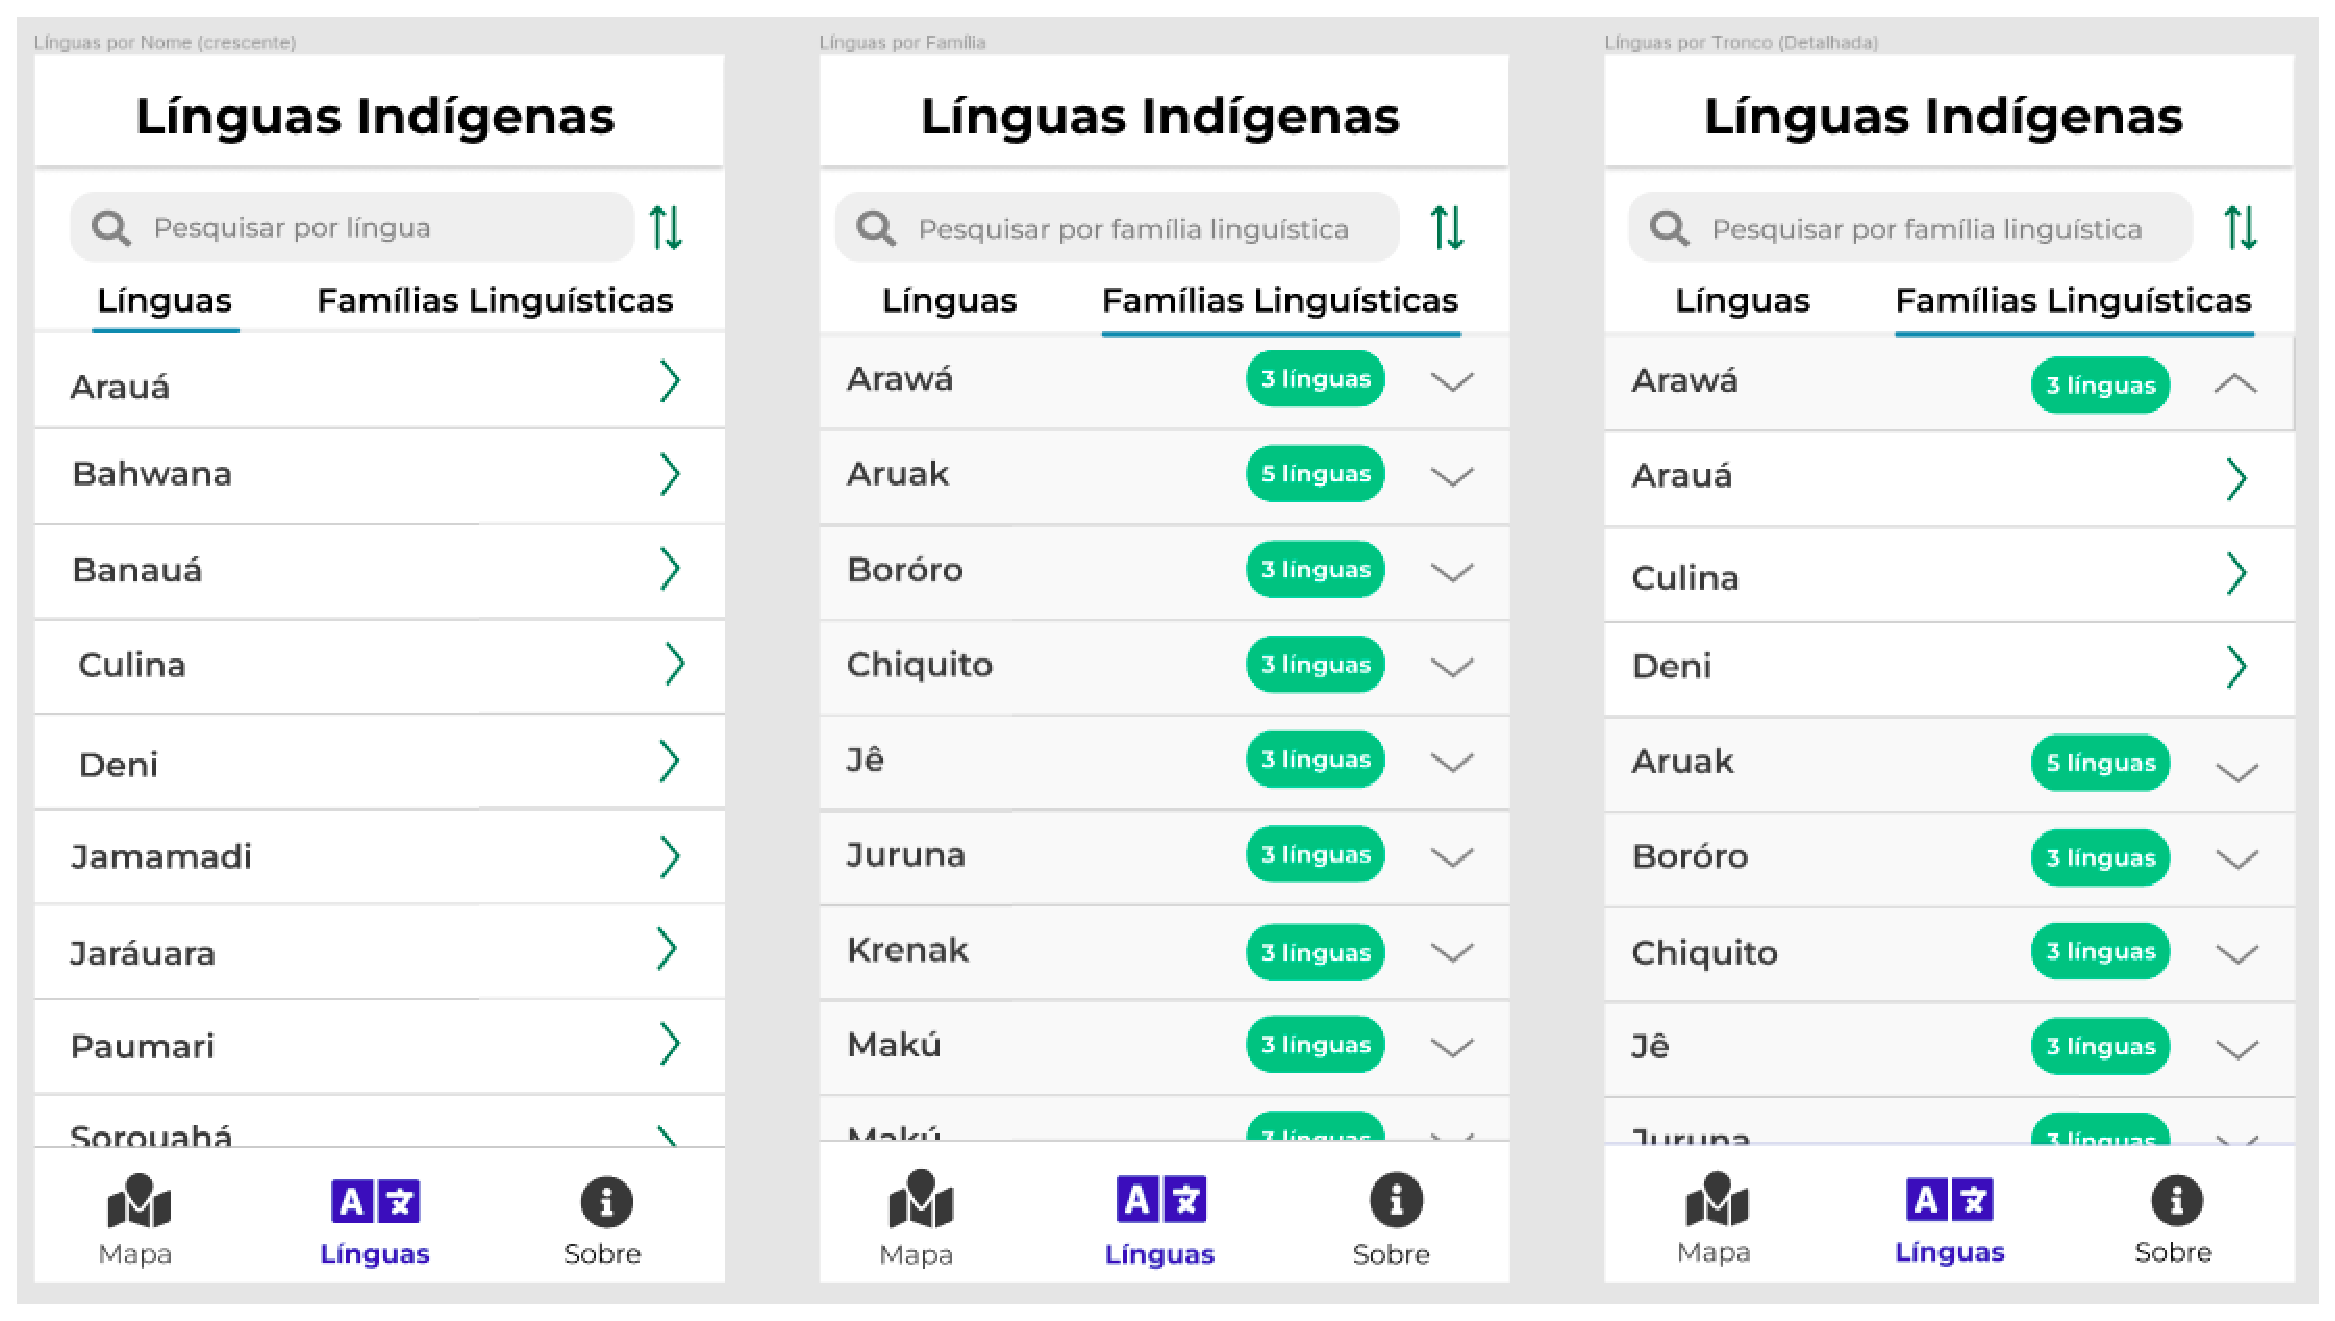
\includegraphics{figuras/linguas.eps}}
	\begin{tablenotes}[flushleft]
		\centering
		\item \textit{Fonte:} Autora.
	\end{tablenotes}
	\label{fig23}
\end{figure}

A implementação dessa mudança aborda, principalmente, a heurística de "Visibilidade do status do sistema", pois ao substituir o ícone por um texto descritivo, os usuários terão uma compreensão mais clara e explícita da 
funcionalidade disponível, além de poderem visualizar exatamente onde estão através do componente de abas. Em relação a "Correspondência entre o sistema e o mundo real", pode-se pontuar que a funcionalidade se torna mais 
alinhada com a expectativa do usuário, pois através do texto descritivo, podem associar mais facilmente a ação. Além disso, foi adotado o princípio de "Consistência e Padrões", seguindo a utilização de componentes 
reutilizáveis e garantindo a coerência em todo o sistema. 

\subsection{Disposição de Informações}
\label{sec:Disposicao de Informacoes}

Entre as melhorias implementadas no aplicativo, tem-se a reorganização e disposição das informações. A utilização de abas em diferentes telas, como as de línguas, palavras específicas e dicionário. Essas abas foram 
visualmente destacadas quando selecionadas, com o uso de cores distintas para indicar ao usuário em qual seção ele está navegando. Essa mudança proporciona maior visibilidade ao status atual do sistema, tornando mais 
claro para os usuários onde eles estão e qual ação estão realizando.

\begin{figure}[h!]
	\centering
	\caption{Telas da Aplicação - Abas}
	\resizebox{0.85\textwidth}{!}{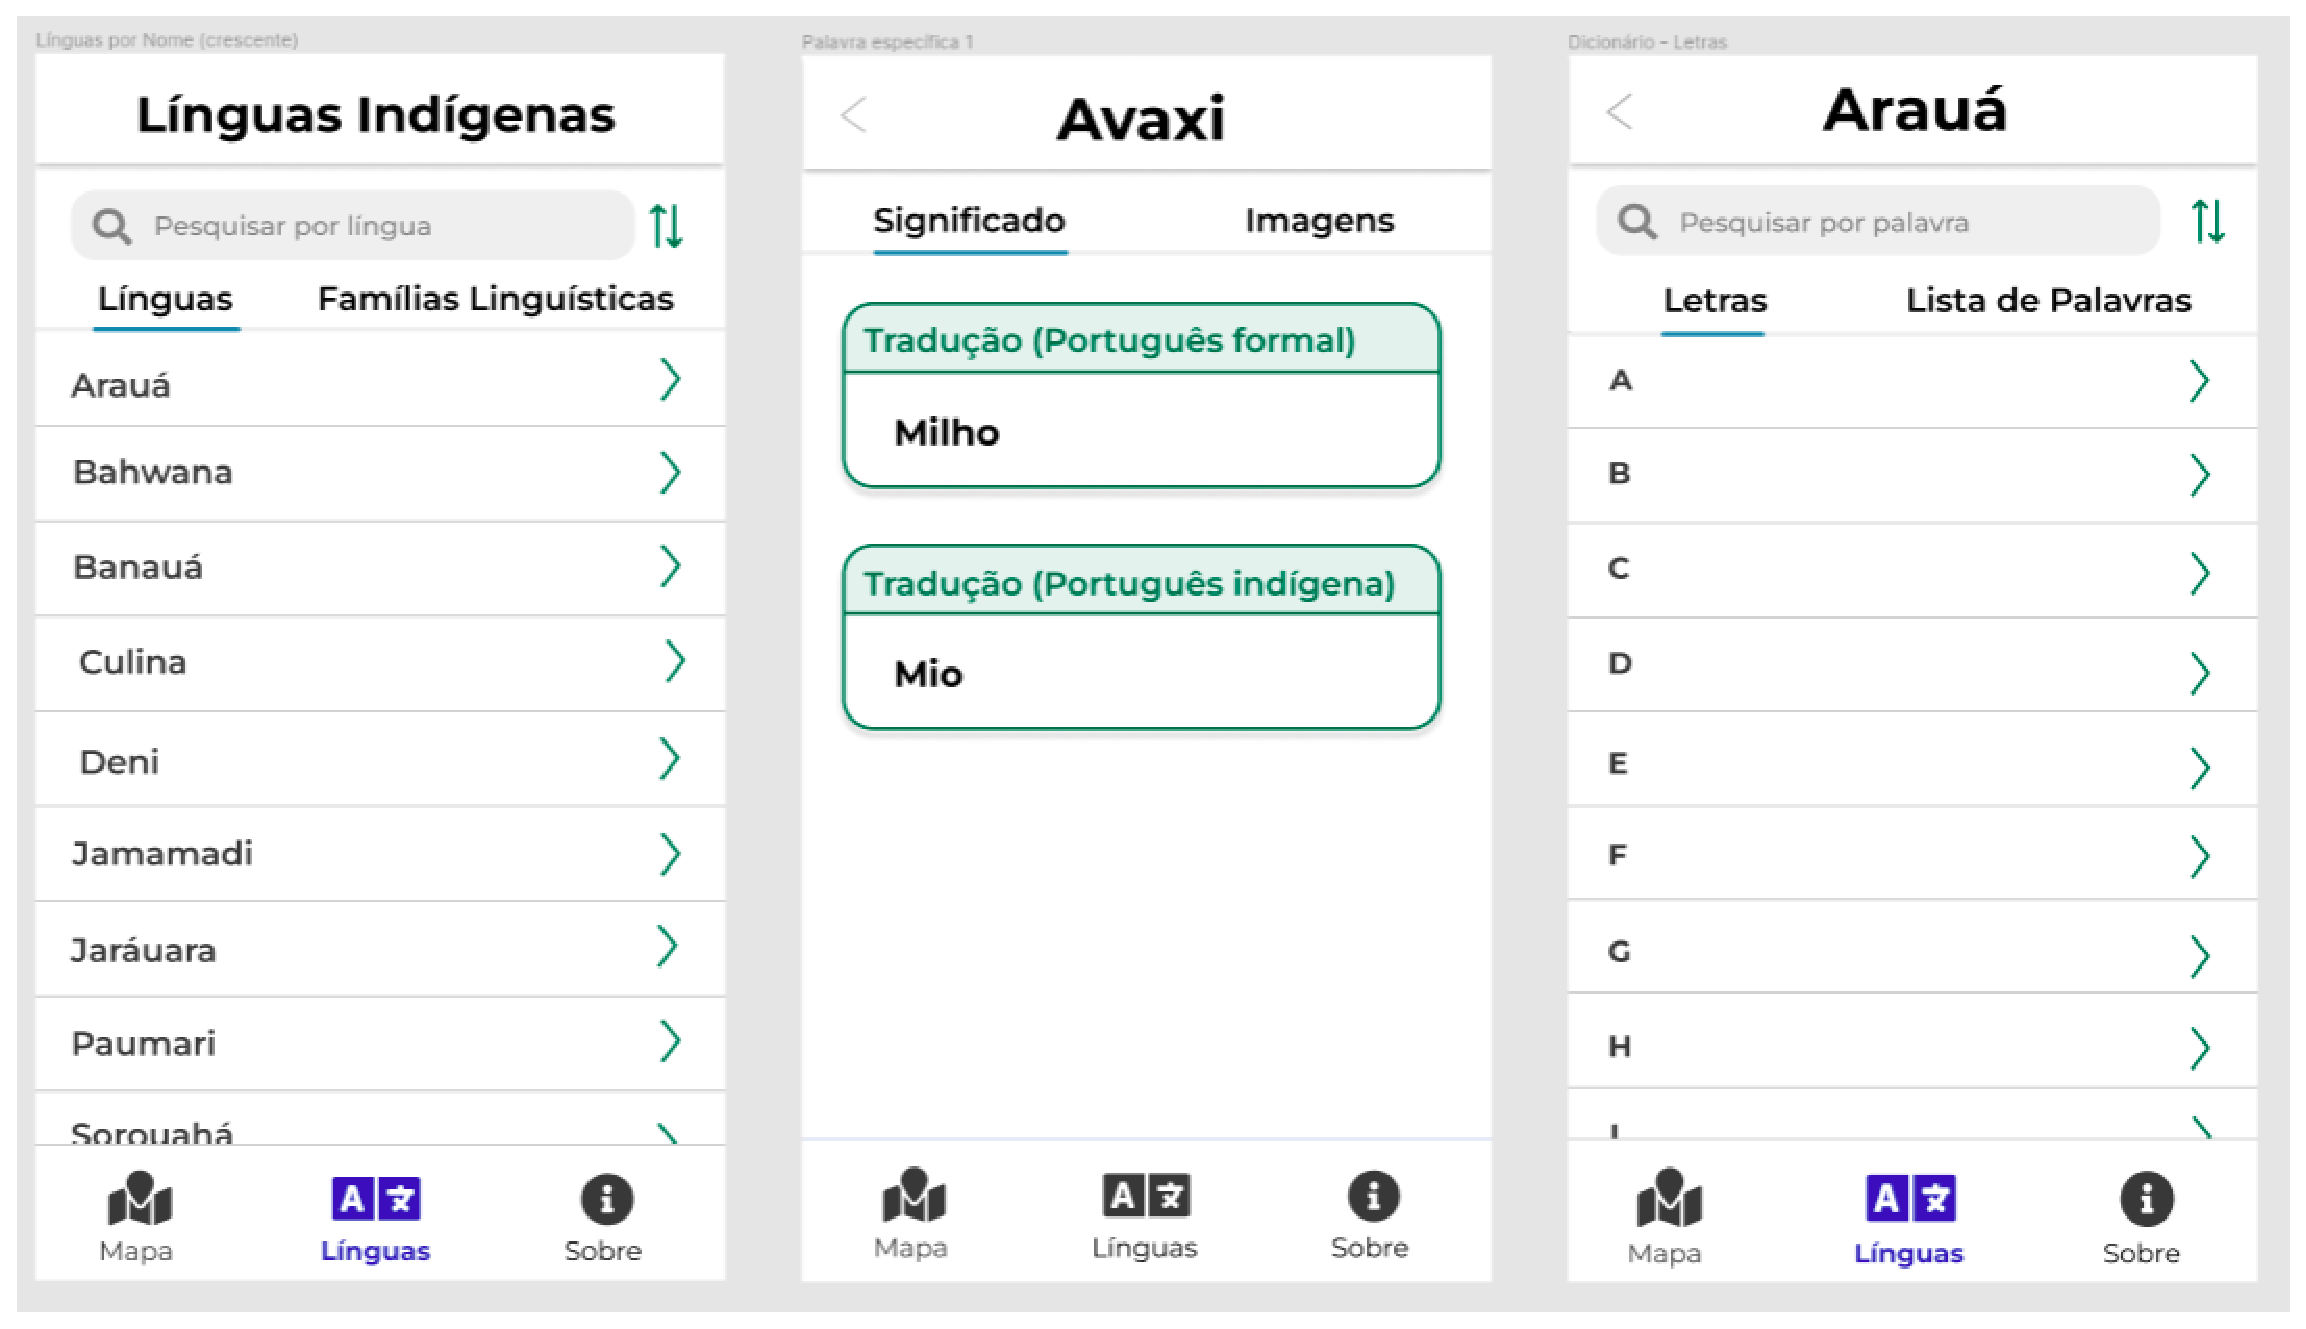
\includegraphics{figuras/abas.eps}}
	\begin{tablenotes}[flushleft]
		\centering
		\item \textit{Fonte:} Autora.
	\end{tablenotes}
	\label{fig24}
\end{figure}

Além disso, para tornar o aplicativo mais atrativo, foram adicionadas novas cores seguindo uma paleta de cores coerente e visualmente agradável. Essas cores foram aplicadas de forma consistente em todo o aplicativo, 
contribuindo para uma experiência visual atraente e harmoniosa. A "Estética e Design Minimalista" foi seguida, buscando evitar sobrecarregar os usuários com informações desnecessárias, focando apenas no essencial.

\begin{figure}[h!]
	\centering
	\caption{Componentes da Aplicação}
	\resizebox{0.85\textwidth}{!}{\includegraphics{figuras/componentes.eps}}
	\begin{tablenotes}[flushleft]
		\centering
		\item \textit{Fonte:} Autora.
	\end{tablenotes}
	\label{fig25}
\end{figure}

Outra melhoria importante foi a adição de informações sobre como contribuir com o aplicativo. Essa inclusão permite que os usuários tenham conhecimento sobre como podem participar ativamente do desenvolvimento do aplicativo, 
fornecendo \textit{feedback}, relatando erros e contribuindo com sugestões. Tal melhoria permite maior "Liberdade e Controle do Usuário" na aplicação, permitindo que eles participem ativamente no desenvolvimento e aprimoramento 
das informações presentes.

Por fim, também foi definido de forma mais clara e explícita o que é o português indígena, fornecendo uma definição compreensível aos usuários. Essa informação fornece uma forma de "Ajuda e Documentação" aos usuários, promovendo uma melhor 
compreensão e orientação durante o uso do aplicativo.


\section{Segundo Ciclo de Testes}
\label{sec:Segundo Ciclo}
O processo de \textit{design} segue uma abordagem iterativa, ou seja, é uma atividade contínua envolvendo \textit{feedback} constante dos usuários e melhorias incrementais ao longo do tempo. \citeonline{usabilitytest} 
reconhece que nem sempre é possível envolver usuários novos a cada iteração e que é possível, com os mesmos usuários, descobrir problemas persistentes e validar melhorias implementadas. 

Após o primeiro estudo, com cinco participantes, ter encontrado alguns problemas de usabilidade, o \textit{design} foi redesenhado\footnote{Protótipo com melhorias. Disponível em: \url{https://shorturl.at/ryEOR}(último acesso: Julho 2023)}. 
A segunda rodada de testes com cinco usuários visa mapear os demais problemas de usabilidade que não foram encontrados na primeira rodada de testes. O segundo estudo poderá aprofundar a usabilidade da estrutura fundamental do site, avaliando questões como arquitetura da informação, fluxo de tarefas e correspondência 
com as necessidades do usuário \cite{usabilitytest}.

\subsubsection{Resultado do Segundo Ciclo de Testes}
\label{sec:Resultado do Segundo Ciclo de Testes}
A Tabela \ref{tab07} apresenta o tempo gasto por cada testador durante o teste de usabilidade separado por funcionalidade.

\begin{table}[h!]
	\centering
	\caption{Tempo gasto por testador - Segundo ciclo de testes}
	\label{tab07}
	\begin{tabular}{l|l|l|l|l|l}
	\hline
	Fucionalidade & Testador 1 & Testador 2 & Testador 3 & Testador 4 & Testador 5 \\ 	\hline
	F01                   & 8.8s     & 12s     & 5,1s      & 9.4s       & 20.1s      \\
	F02                   & 8.4s        & 11.8s      & 8.8s      & 13.9s    & 14.2s     \\
	F03                   & 20.7s        & 4.5s      & 32.9s      & 100s     & 44.4s     \\
	F04                   & 16.1s        & 21.1s     & 89.9s     & 48.1s     & 13.8s     \\
	F05                   & 14.8s      & 18.8s      & 10.8s     & 33s     & 62.7s     \\
	F06                   & 18.4s     & 11.1s      & 14.6s     & 14.4s     & 18.2s     \\
	F07                   & 18.9s     & 20.8s      & 25s     & 21s    & 52.9s       \\ 	\hline
	\end{tabular}
	\begin{tablenotes}[flushleft]
		\centering
		\item \textit{Fonte:} Maze. Disponível em: \url{https://app.maze.co/report/Novo-Multilind/hsf4hljyldyqs/intro}.
	  \end{tablenotes}
\end{table}

A tabela presente no Google Sheets apresenta as avaliações obtidas por meio do formulário \textit{Attrakdiff} aplicado aos testadores do aplicativo. Além disso, as Figuras \ref{fig26} e \ref{fig27} ilustram a média de respostas geral e a média 
de respostas separadas pelas quatro dimensões principais, respectivamente.

\begin{figure}[h!]
	\centering
	\caption{Média Geral \textit{Attrakdiff} - Segundo Ciclo de Testes}
	\resizebox{0.8\textwidth}{!}{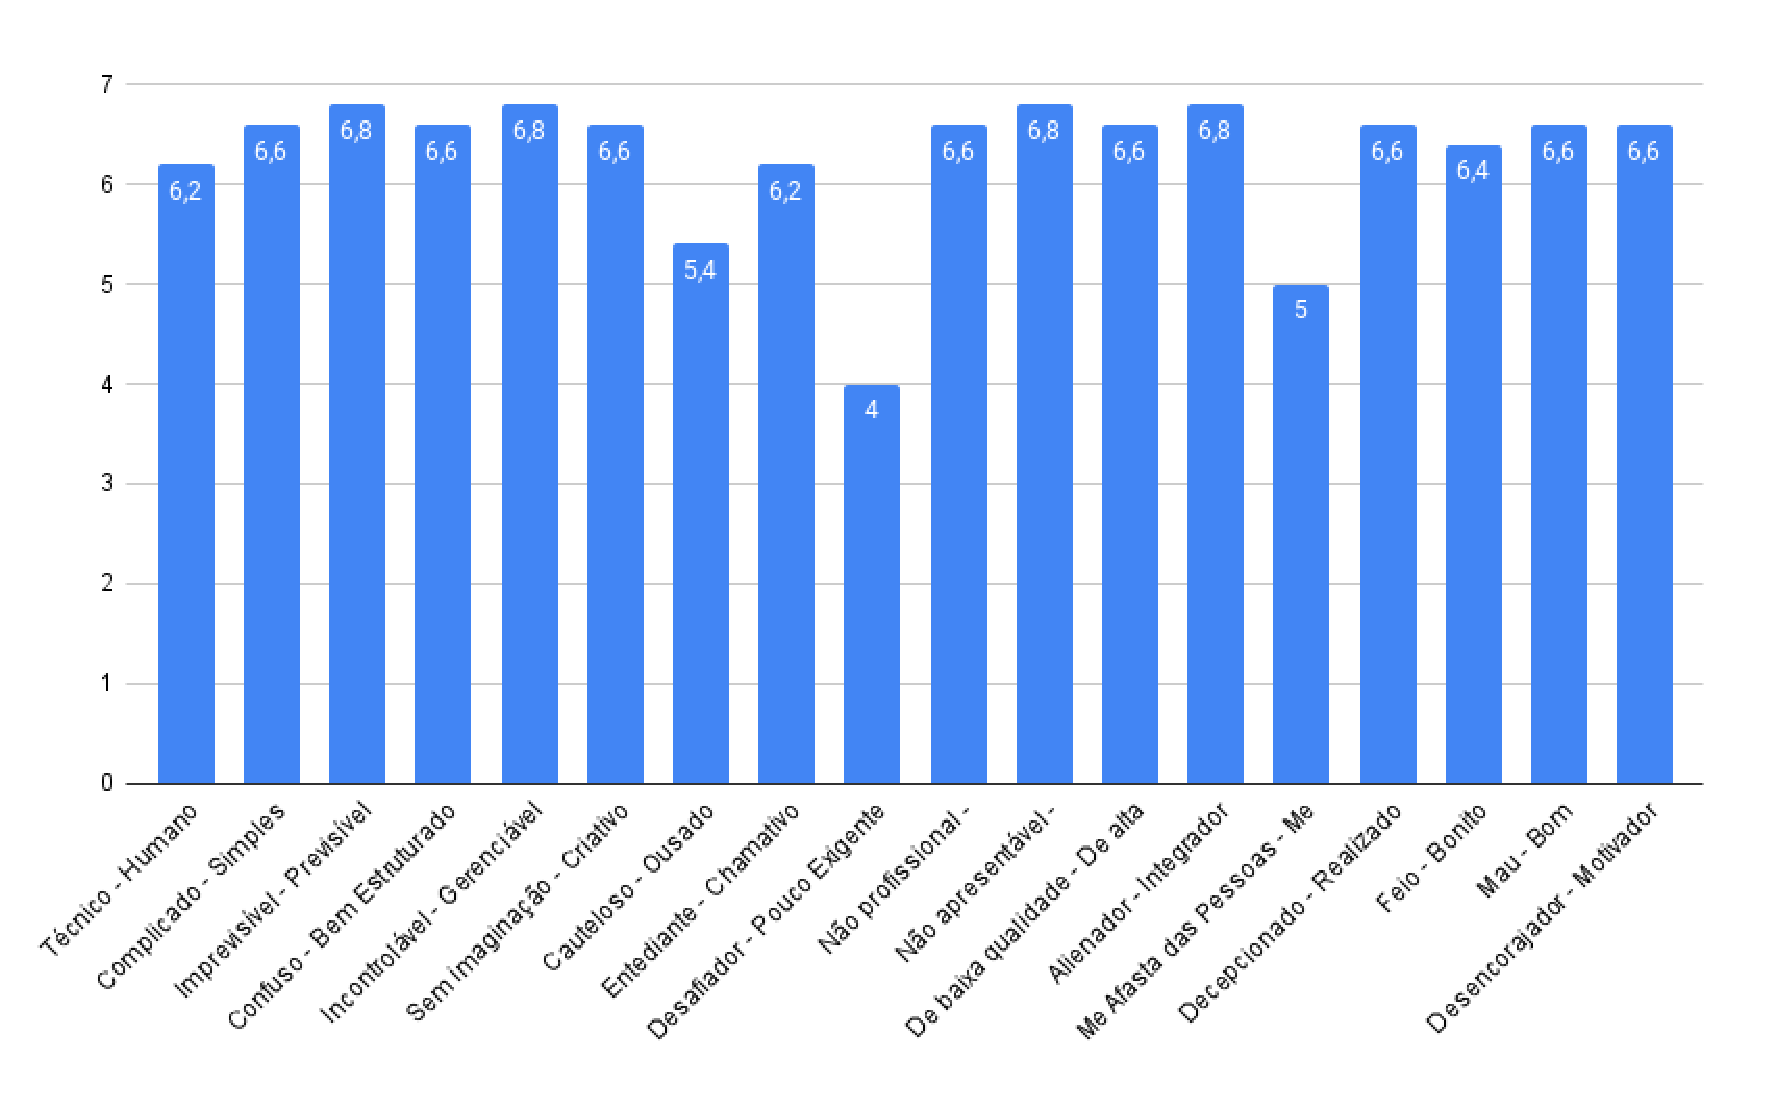
\includegraphics{figuras/media-geral1.eps}}
	\begin{tablenotes}[flushleft]
		\centering
		\item \textit{Fonte:} Autora.
	\end{tablenotes}
	\label{fig26}
\end{figure}

\begin{figure}[h!]
	\centering
	\caption{Média \textit{Attrakdiff} por dimensões- Segundo Ciclo de Testes}
	\resizebox{0.8\textwidth}{!}{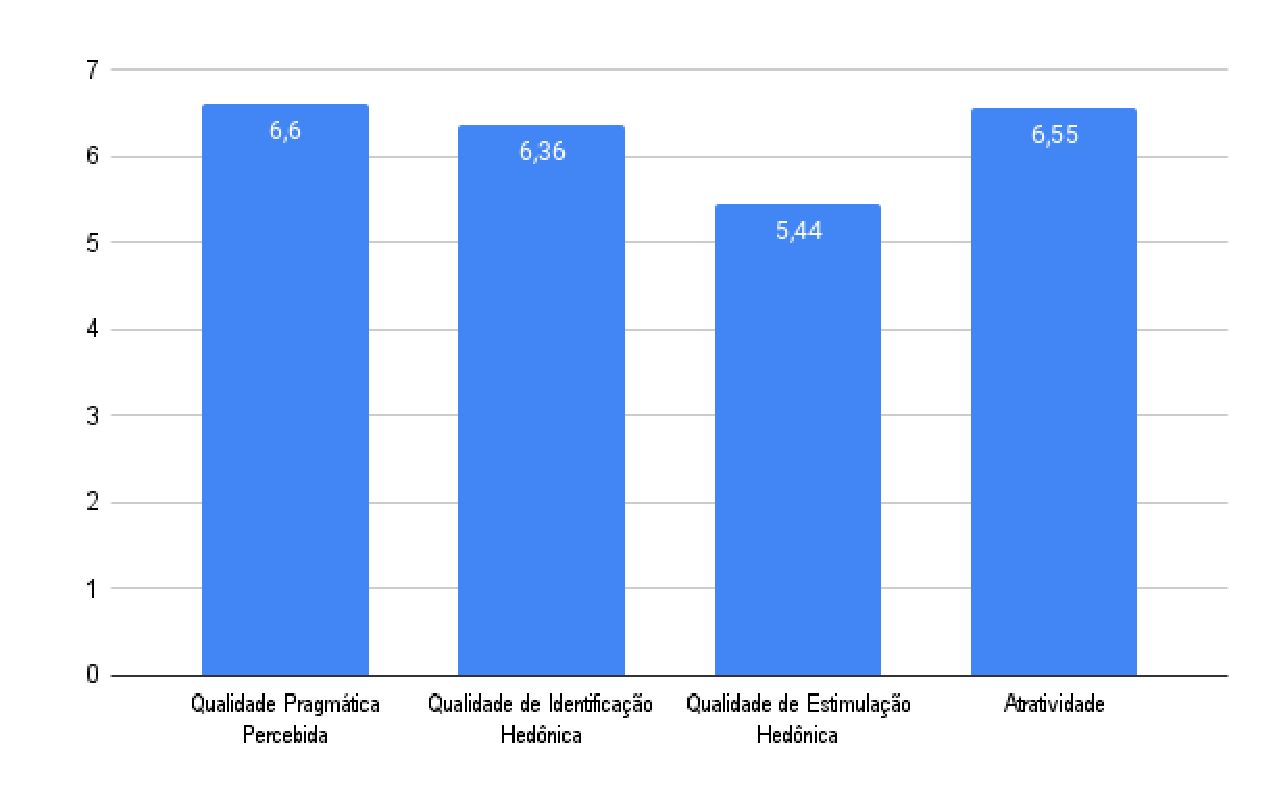
\includegraphics{figuras/media-separada1.eps}}
	\begin{tablenotes}[flushleft]
		\centering
		\item \textit{Fonte:} Autora.
	\end{tablenotes}
	\label{fig27}
\end{figure}

Os usuário relataram melhor entendimento da aplicação devido ao passo a passo inicial, além da validação da mudança dos fluxos no aplicativo, que se demonstraramm mais intuitivos. Os dados revelam melhoria nas quatro dimensões principais do \textit{AttrakDiff}, 
que avalia a experiência do usuário. A Qualidade Pragmática Percebida, que mede o grau de sucesso e esforço que os usuários têm ao utilizar o aplicativo para atingir seus objetivos, teve uma melhora significativa, anteriormente de 5,48 para 6,6. Em relação a 
Qualidade Hedônica-Identidade, pode-se notar uma melhoria considerável, atingindo 6,36. Essa dimensão representa o grau de identificação da aplicação com o usuário. Já a Qualidade Hedônica-Estímulo, indica a quantidade de suporte que o produto oferece ao usuário 
para desenvolver, estimular e aumentar a motivação. Uma pequena melhora pode ser notada, de 5,2 para 5,44. E por fim, foi medida a Atratividade da aplicação, que representa uma classificação global e melhorou em 0,4 pontos, chegando a 6,55.

O aumento mais significativo em relação as estatísticas foi na Qualidade Pragmática Percebida e refere-se à percepção do usuário em relação à funcionalidade, eficiência e facilidade de uso. O que indica facilidade dos usuários em atender às suas necessidades e 
objetivos.

Possíveis melhorias também foram pontuadas durante o segundo ciclo de testes:

\begin{itemize}
	\item Português Indígena: Alguns usuários expressaram preocupação em relação a tradução para o português indígena, visto que não se trata de uma língua única, mas sim uma variação do português brasileiro que depende de alguns fatores, como contato linguístico com outros 
	povos, região do Brasil, identidade cultural e grau de preservação da língua nativa.
	\item Participação Coletiva: Com objetivo de maior participação de falantes das línguas, a opção de reportar em caso de erro de tradução ou inconsistência foi sugerida. Tal funcionalidade visa aumentar a confiabilidade dos dados presentes no aplicativo e incentivar a 
	participação dos povos indígenas na documentação das línguas.
	\item Pronúncia de Palavras: A língua oral é a principal forma de comunicação e expressão cultural para muitos povos indígenas, por isso a adição de uma funcionalidade de pronúncia pode ser uma ótima maneira de ajudar os usuários a compreender palavras de maneira mais clara 
	e precisa.
\end{itemize}

\section{Backlog de Melhorias}
\label{sec:Backlog de Melhorias}
Foi elaborado um \textit{Product Backlog}, contendo histórias de usuário, a partir da concepção do protótipo e das melhorias pontuadas, para orientar o desenvolvimento deste projeto. Além disso, a técnica MoSCoW foi utilizada para realizar a priorização. Seguindo essa classificação, 
os requisitos são categorizados como \textit{Must Have}, \textit{Should Have}, \textit{Could Have} e \textit{Won't Have} \cite{miranda2021}. 


\begin{table}[h!]
	\centering
	\caption{\textit{Backlog}}
	\label{tab08}
	\begin{tabularx}{\textwidth}{p{1cm}|p{12cm}|p{1cm}}
	\hline
	ID   & História de Usuário                                                                                                                                                                                                   & Priorização \\ \hline
	US01 & Eu, como usuário, desejo ter um processo de \textit{onboarding} no aplicativo que me guie de forma clara e intuitiva pelas funcionalidades e navegação disponíveis.                                                            & \textit{Must}        \\
	US02 & Eu, como usuário, desejo visualizar línguas por família linguística por meio de abas na tela de Línguas                                                                                                               & \textit{Must}        \\
	US03 & Eu, como usuário, desejo ter a opção de trocar de abas em vez de mudar de página para visualizar imagens e traduções relativas a uma palavra específica, facilitando o acesso.                                        & \textit{Must}        \\
	US04 & Eu, como usuário, desejo ter uma forma fácil e acessível de obter informações sobre como posso contribuir para a base de dados do aplicativo.                                                                         & \textit{Must}        \\
	US05 & Eu, como usuário, desejo ter acesso direto à lista de palavras no dicionário, para facilitar a navegação e pesquisa.																									 & \textit{Must}        \\
	US06 & Eu, como usuário, desejo obter uma explicação clara sobre o que é o português indígena, a fim de compreender melhor sua definição e significado.                                                                      & \textit{Must}        \\
	US07 & Eu, como usuário, desejo que o design da aplicação seja mais atraente e visualmente agradável, através da adição de mais cores que complementem a interface.                                                          & \textit{Should}      \\
	US08 & Eu, como usuário, desejo obter informações precisas sobre o nome da língua do português indígena que está relacionada a uma língua específica, a fim de compreender melhor sua classificação linguística. 			 & \textit{Should}      \\
	US09 & Eu, como usuário, desejo ter a opção de relatar erros ou inconsistências nas traduções e imagens das palavras, a fim de contribuir para a consistência das informações apresentadas.                                  & \textit{Should}      \\
	US10 & Eu, como usuário, desejo ter a opção de ouvir a pronúncia correta das palavras no aplicativo, a fim de melhorar minha compreensão e pronúncia adequada.                                                               & \textit{Should}      \\ \hline
	\end{tabularx}
\end{table}

\section{Resumo do Capítulo}
\label{sec:Resumo Proposta}
No capítulo em questão, o contexto no qual o trabalho se propõe a contribuir é revisado e a proposta do Trabalho de Conclusão de Curso é apresentada. A seção de \hyperref[sec:Contextualização]{Contextualização} fornece informações sobre o domínio no qual o estudo está inserido. Além disso, 
a seção de \hyperref[sec:Detalhamento da Aplicacao]{Detalhamento da Aplicação} é apresentada para garantir uma adequada compreensão da aplicação Multilind. A \hyperref[sec:Prova de Conceito]{Prova de Conceito} descreve em detalhes como os testes de usabilidade serão conduzidos. O \hyperref[sec:Primeiro Ciclo]{Primeiro Ciclo de Teste} 
detalha os métodos e resultados dos testes realizados, enquanto a seção de \hyperref[sec:Melhorias Propostas]{Melhorias Propostas} aborda os aspectos trabalhados na versão com melhorias. O \hyperref[sec:Segundo Ciclo]{Segundo Ciclo de Teste} apresenta os resultados finais dos testes realizados na versão aprimorada. 
Além disso, a seção de \hyperref[sec:Backlog]{Backlog de Melhorias} apresenta uma lista priorizada das funcionalidades que serão implementadas. 